%NEURAL PRESY ;)

%----------------------------------------------------------------------------------------
%   PACKAGES AND THEMES
%----------------------------------------------------------------------------------------

\documentclass{beamer}

\mode<presentation> {

% The Beamer class comes with a number of default slide themes
% which change the colors and layouts of slides. Below this is a list
% of all the themes, uncomment each in turn to see what they look like.

%\usetheme{default}
%\usetheme{AnnArbor}
%\usetheme{Antibes}
%\usetheme{Bergen}
\usetheme{Berkeley}
%\usetheme{Berlin}
%\usetheme{Boadilla}
%\usetheme{CambridgeUS}
%\usetheme{Copenhagen}
%\usetheme{Darmstadt}
%\usetheme{Dresden}
%\usetheme{Frankfurt}
%\usetheme{Goettingen}
%\usetheme{Hannover}
%\usetheme{Ilmenau}
%\usetheme{JuanLesPins}
%\usetheme{Luebeck}
%\usetheme{Madrid}
%\usetheme{Malmoe}
%\usetheme{Marburg}
%\usetheme{Montpellier}
%\usetheme{PaloAlto}
%\usetheme{Pittsburgh}
%\usetheme{Rochester}
%\usetheme{Singapore}
%\usetheme{Szeged}
%\usetheme{Warsaw}

% As well as themes, the Beamer class has a number of color themes
% for any slide theme. Uncomment each of these in turn to see how it
% changes the colors of your current slide theme.

%\usecolortheme{albatross}
%\usecolortheme{beaver}
%\usecolortheme{beetle}
%\usecolortheme{crane}
%\usecolortheme{dolphin}
%\usecolortheme{dove}
%\usecolortheme{fly}
%\usecolortheme{lily}
%\usecolortheme{orchid}
%\usecolortheme{rose}
%\usecolortheme{seagull}
%\usecolortheme{seahorse}
%\usecolortheme{whale}
%\usecolortheme{wolverine}

%\setbeamertemplate{footline} % To remove the footer line in all slides uncomment this line
%\setbeamertemplate{footline}[page number] % To replace the footer line in all slides with a simple slide count uncomment this line

\setbeamertemplate{navigation symbols}{} % To remove the navigation symbols from the bottom of all slides uncomment this line
}

\usepackage{graphicx} % Allows including images
\usepackage{booktabs} % Allows the use of \toprule, \midrule and \bottomrule in tables
\usepackage{caption}
\usepackage{subcaption}
\usepackage{algorithm,algorithmic}

% tikz and associated macros
\usepackage{tikz}
\usepackage{tikz-cd}

\usepackage{pgfplots}
\def\layersep{2cm}
\def\nodesep{0.25cm}
\newcommand*{\Scale}[2][4]{\scalebox{#1}{$#2$}}%
\newcommand*{\Resize}[2]{\resizebox{#1}{!}{$#2$}}%
\newcommand\sep{1.9cm}
\newcommand\height{0.9cm}
\usetikzlibrary{decorations.pathmorphing, backgrounds}
\tikzset{snake it/.style={decorate, decoration=snake}}

%
%

% math
\usepackage{amsthm}
\usepackage{amsmath}
\usepackage{amssymb}
\usepackage{mathabx}

\numberwithin{equation}{subsection}
\numberwithin{theorem}{subsection}

\DeclareSymbolFont{cmlargesymbols}{OMX}{cmex}{m}{n}
\let\sumop\relax
\DeclareMathSymbol{\sumop}{\mathop}{cmlargesymbols}{"50}


\def\reals{{\mathbb R}}
\def\torus{{\mathbb T}}
\def\integers{{\mathbb Z}}
\def\rationals{{\mathbb Q}}
\def\expect{\mathop{{\mathbb{E}}}}
\def\tens{\mathop{{\bigotimes}}}
\def\naturals{{\mathbb N}}
\def\complex{{\mathbb C}\/}
\def\distance{\operatorname{distance}\,}
\def\support{\operatorname{support}\,}
\def\dist{\operatorname{dist}\,}
\def\Span{\operatorname{span}\,}
\def\degree{\operatorname{degree}\,}
\def\kernel{\operatorname{kernel}\,}
\def\dim{\operatorname{dim}\,}
\def\codim{\operatorname{codim}}
\def\trace{\operatorname{trace\,}}
\def\dimension{\operatorname{dimension}\,}
\def\codimension{\operatorname{codimension}\,}
\def\kernel{\operatorname{Ker}}
\def\Re{\operatorname{Re\,} }
\def\Im{\operatorname{Im\,} }
\def\eps{\varepsilon}
\def\lt{L^2}
\def\bull{$\bullet$\ }
\def\det{\operatorname{det}}
\def\Det{\operatorname{Det}}
\def\diameter{\operatorname{diameter}}
\def\symdif{\,\Delta\,}
\newcommand{\norm}[1]{ \|  #1 \|}
\newcommand{\set}[1]{ \left\{ #1 \right\} }
\def\suchthat{\mathrel{}\middle|\mathrel{}}
\def\one{{\mathbf 1}}
\def\cl{\text{cl}}

\def\newbull{\medskip\noindent $\bullet$\ }
\def\nobull{\noindent$\bullet$\ }
\def\defeq{\stackrel{\text{def}}{=}}


\def\scriptf{{\mathcal F}}
\def\scriptq{{\mathcal Q}}
\def\scriptg{{\mathcal G}}
\def\scriptm{{\mathcal M}}
\def\scriptb{{\mathcal B}}
\def\scriptc{{\mathcal C}}
\def\scriptt{{\mathcal T}}
\def\scripti{{\mathcal I}}
\def\scripte{{\mathcal E}}
\def\scriptv{{\mathcal V}}
\def\scriptw{{\mathcal W}}
\def\scriptu{{\mathcal U}}
\def\scriptS{{\mathcal S}}
\def\scripta{{\mathcal A}}
\def\scriptr{{\mathcal R}}
\def\scripto{{\mathcal O}}
\def\scripth{{\mathcal H}}
\def\scriptd{{\mathcal D}}
\def\scriptl{{\mathcal L}}
\def\scriptn{{\mathcal N}}
\def\scriptp{{\mathcal P}}
\def\scriptk{{\mathcal K}}
\def\scriptP{{\mathcal P}}
\def\scriptj{{\mathcal J}}
\def\scriptz{{\mathcal Z}}
\def\scripts{{\mathcal S}}
\def\scriptx{{\mathcal X}}
\def\scripty{{\mathcal Y}}
\def\frakv{{\mathfrak V}}
\def\frakG{{\mathfrak G}}
\def\frakB{{\mathfrak B}}
\def\frakC{{\mathfrak C}}



%----------------------------------------------------------------------------------------
%   TITLE PAGE
%----------------------------------------------------------------------------------------

\title[OpenBrain]{OpenBrain: Backpropagation Free RL}

\author[Guss \& Zhong et. al]{
\includegraphics[height=2cm,width=2cm]{BlueGold_fill_small.png}\\   Guss,  Zhong  \\ Kuznetsov,  \ Kumar,  Golmant, Johansen,  Bartlett}
\date{April 22, 2016} % Date, can be changed to a custom date
\makeatletter
\newcommand{\verbatimfont}[1]{\renewcommand{\verbatim@font}{\ttfamily#1}}
\makeatother
\begin{document}

\begin{frame}
\titlepage
\end{frame}

\addtobeamertemplate{frametitle}{}{%
\begin{tikzpicture}[remember picture,overlay]
\node[anchor=north east,yshift=10pt] at (current page.north east) {
\includegraphics[height=2cm]{White_outline_small_name_transparent.png}};
\end{tikzpicture}}

\begin{frame}

\begin{center}
\Huge
\end{center}


\frametitle{Overview}
\tableofcontents
\end{frame}

\begin{frame}
\frametitle{The Problem}
    \Huge{\centerline{Can we decentralize }}
    \Huge{\centerline{deep reinforcement learning?}}
\end{frame}

\begin{frame}
\frametitle{The Problem}
    \Huge{\centerline{Can we decentralize }}
    \Huge{\centerline{deep reinforcement learning?}}
    \Huge{\centerline{\textbf{Yes.} Here's how. }}
\end{frame}



\section{Results}
\begin{frame}
\frametitle{Results}
      \begin{columns}
      \begin{column}{0.6\textwidth}

  \textbf{The Training Regime}
  \begin{enumerate}
  \item We can train every neuron \textbf{simultaneously} without BP.
  \item There is no "extra" $Q$ network, just $2n$ parameters!
  \item Could be biologically plausible (certainly more reasonable than BP)
  \item Linear critic $\iff$ \emph{compatability} $\iff$ no bias in $Q^n$
  \end{enumerate}
      \end{column}
      \begin{column}{0.4\textwidth}
      \begin{figure}
          \begin{centering}
            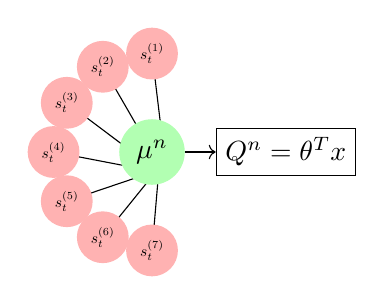
\begin{tikzpicture}
              \foreach \a in {1,2,...,7}{
              \path[draw, ->] (\a*360/6: 0.25cm)  -- (\a*360/12 + 60: 1.5cm-0.25cm) node[circle, fill=red!30, scale=0.8] {$\Scale[0.7]{s_t^{(\a)}}$};
              }
            \node[circle, style=dashed, fill=green!30] (A) {$\mu^n$};
            \node[rectangle] at (1.7,0) [draw] (B) {$Q^n = \theta^Tx$};
            \draw[->] (A) edge (B);
          \end{tikzpicture}
          \end{centering}
          \caption{A linear critic for $\mu^n$ }
      \end{figure}

      \end{column}
    \end{columns}

\end{frame}


\begin{frame}[fragile]
    \frametitle{Theorem 1}
    \begin{theorem}[Neurocomputational Decompostion]\label{thm:ncomp}
      Let $E$ be an environment and $\scriptn$ be a neurocomputational agent. Then there exists a set of agent environment pairs $\mathfrak{D}_\scriptn \defeq \{(E^n, \mu^n)\}_{n\in \scriptn}$ such that for every $n \in \scriptn$, the following diagram commutes
        \begin{equation}\label{eq:sub_env_com}
            \begin{tikzcd} %THe diagram for Q function decomposition.
  %-------------------------------------------------------------------------------------%
          \scriptv  \times \scripts \arrow{r}{\mu\circ\pi_2}
               \arrow{d}
                 {\pi_1  \times\epsilon \circ \pi_2}  &[+25pt]  \scripta    \\
  %-------------------------------------------------------------------------------------%%
            \overbrace{\scriptv \times \scriptv}^{(v_{t},\epsilon(s_t))}
                        \arrow{r}{D}
                                    \arrow[pos = 0.7]{rd}[swap]{\mu^n\circ\pi_1 + \pi_n \circ \pi_2}
                        & \overbrace{\scriptv}^{v_{t+1}}
                                              \arrow[two heads, pos=0.8]
                                                {d}
                                                {\pi_n}
                                              \arrow{u}{\delta} \\
  %%%%%%%%%%%%%%%%%%%%%%%%%%%%%%%%%%%%%%%%%%%%%%%%%%%%%%%%%%%%%%%%%%%%%%%%%%%%%%%%%%%%%%%
    &\reals
           \end{tikzcd}
        \end{equation}
    \end{theorem}
\end{frame}

\begin{frame}
    \frametitle{Theorem 2}
    \begin{theorem}
        If $\scriptn$ is a nuerocomputational agent in $E$, then policy gradient for $\mu$ agrees with the simultaneous policy gradients of its decomposition; that is for every $(E^n, \mu^n) \in \mathfrak{D}_\scriptn$
        \begin{equation}
            \nabla_{K^n} Q^{\mu^n}(v,\alpha)\Big|_{v=v_t,\alpha=\mu^n(v_t)} =\nabla_{K^n} Q^{\mu}(s,a)\Big|_{s=s_t,a=\mu(s_t)}
        \end{equation}
        for every time step $t$, where $K^n$ is the nth column of the linear voltage graph transition matrix, i.e. the weights of the connections from all neurons to neuron $n.$
    \end{theorem}
\end{frame}
\begin{frame}
  \frametitle{Experiments}
  \textbf{Experiment 1.}
  \begin{enumerate}
    \item Test if training $\mu$ with the full $Q^n$ $\implies$ each $\mu^n$ acting optimal to $Q^n$
    \item Is it true in practice that $\nabla_{W^{(n)}} Q^{n}(\mu^n) = \left(\nabla_{W} Q^\mu(\mu)\right)^{(n)}$?
  \end{enumerate}
    \textbf{Experiment 2.}
    \begin{enumerate}
      \item Train $\mu^n$ using $Q^n$ $\implies$ $Q$ optimal?
    \end{enumerate}
        \textbf{Experiment 3.}
    \begin{enumerate}
      \item Beat the state of the art in Atari 2600 environments!
    \end{enumerate}
\end{frame}
% \begin{frame}
%     \frametitle{Experiment 1}
%     % \textbf{Experiment 1}
%     Compare subcritic Q-values to Q-values of the critic.
% \end{frame}
\begin{frame}
    \frametitle{Experiment 1 Results}
    \begin{column}{0.5\textwidth}
        Subcritic Layer 0 Neuron 3
        % TODO Insert here
        
\includegraphics[height=2cm,width=2cm]{BlueGold_fill_small.png}
    \end{column}
    \begin{column}{0.5\textwidth}
        Network Critic Q value
        % TODO Insert here
        
\includegraphics[height=2cm,width=2cm]{BlueGold_fill_small.png}
    \end{column}
\end{frame}
\begin{frame}
    \frametitle{Experiment 2}
    \textbf{Goal:} Use the subcritics to train the actor network
    Progress: currently tweaking experiment.
\end{frame}
%------------------------------------------------

\begin{frame}
\Huge{\centerline{Questions?}}
\Small\centerline{wguss@berkeley.edu}
\end{frame}

%----------------------------------------------------------------------------------------

\end{document}
